\documentclass[12pt]{article}
\usepackage{float}
\usepackage[dvipsnames]{xcolor}
\usepackage{dingbat, tikz}
\usepackage{amsfonts,amsmath, color, fullpage, graphicx, mathtools, empheq, amsthm, amssymb}
\usepackage{wasysym}
\usepackage{thmtools}
\usepackage{listings}
\usepackage[framed]{mcode}

\newtheorem{problem}{Problem}
\newtheorem{lemma}{Lemma}

% to put colored box around theorem\problem\lemma etc
\usepackage{tcolorbox}
% make custom box so I can specify the color
\newtcolorbox{mybox}[3][]
{
  colframe = #2!25,
  colback  = #2!10,
  coltitle = #2!20!black,  
  title    = #3,
  #1,
}

%To allow for matrix larger than 10x10
\setcounter{MaxMatrixCols}{11}

%To set thumbs up as QED symbol
\renewcommand{\qedsymbol}{\begingroup \color{blue} \rightthumbsup \endgroup}

%To make a new command for an asterisk in a circle
\newcommand{\circlesign}[1]{ 
    \mathbin{
        \mathchoice
        {\buildcirclesign{\displaystyle}{#1}}
        {\buildcirclesign{\textstyle}{#1}}
        {\buildcirclesign{\scriptstyle}{#1}}
        {\buildcirclesign{\scriptscriptstyle}{#1}}
    } 
}
\newcommand\buildcirclesign[2]{%
    \begin{tikzpicture}[baseline=(X.base), inner sep=0, outer sep=0]
    \node[draw,circle] (X)  {\ensuremath{#1 #2}};
    \end{tikzpicture}%
}

%To use a border matrix with brackets
\usepackage{etoolbox}
\let\bbordermatrix\bordermatrix
\patchcmd{\bbordermatrix}{8.75}{4.75}{}{}
\patchcmd{\bbordermatrix}{\left(}{\left[}{}{}
\patchcmd{\bbordermatrix}{\right)}{\right]}{}{}

%To make tet in an equation smaller
\newcommand*{\Scale}[2][4]{\scalebox{#1}{$#2$}}
%\[\Scale[0.5]{y = \sin^2 x}\] %example of how ot use above command



\def\C{\mathbb{C}}
\def\N{\mathbb{N}}
\def\Q{\mathbb{Q}}
\def\R{\mathbb{R}}
\def\Ts{\mathbb{T}}
\def\Z{\mathbb{Z}}
\def\T{\mathcal{T}}
\def\P{\mathcal{P}}
\title{\underline{Math 226B: Homework \#4}}
\author{\huge Kara Gorman}
\begin{document}
\maketitle


\bigskip\bigskip
\noindent
\begin{problem}
Let $A\in\R^{n\times n}$ be a matrix of the form
$$A = \begin{bmatrix}
0 & 1 \\
I & a \\
\end{bmatrix}$$
where $a\in\R^{n-1}$ and $I$ denotes the $(n-1)\times (n-1)$ identity matrix.  Let $b=e_1$ be the first unit vector of length $n$.
\end{problem}
\begin{itemize}
\item[(a)] Determine the Krylov subspaces $K_k(A,b)$ for all $k=1,2,\dots,d(A,b)$ and show that $d(A,b) = n$.\\

We want to find $K_k(A,b)$ such that:
$$K_k(A,b) = span\{b,Ab,A^2b, \dots, A^{k-1}b\},$$
for $k = 1,2,\dots,d=d(A,b)$.\\
We are given that $b = e_1$, so it follows that:
\begin{align}
Ab &= e_2 \nonumber \\
A^2b &= A(Ab) = A(e_2) = e_3 \nonumber \\
A^3b&= A(A^2b) = A(e_3) = e_4 \nonumber \\
&\vdots \nonumber \\
A^{k-1}b &= e_k \nonumber 
\end{align}
So,
\begin{align}
\Aboxed{K_k(A,b) = span\{e_1, e_2, \dots, e_k\}} \nonumber
\end{align}
for $k=1,2,\dots,d(A,b)$ and show that $d(A,b) = n$.\\

Now, we want to show that $d=d(A,r_0) = n$.  We know that $d = d(A,r_0)=d(A,b)$ is the smallest such $d$ such that the following is true:
$$A^db = c_0 + c_1Ab + c_2A^2b + \dots + c_{d-1}A^{d-1}b \in K_d(A,b).$$
In other words, the grade is the largest number $d = d(A,b)$ such that $K_d(A,b)$ is a linearly independent set.  So clearly, $d = n$ in this case. To show this, let $d = n + 1$.  Then, $K_d(A,b) = span\{e_1, e_2, \dots, e_n, Ae_n\}$, which is not linearly independent.\qed\\


\item[(b)] How many iterations does the MR method with initial guess $x_0 = 0$ need to find the solution of $Ax=b$?\\

From lecture, we know that:
$$x\to x_1 \to \dots \to x_k \to \dots \to x_d = A^{-1}b = x*,$$
where
\begin{align}
d &= d(A,r_0) \nonumber \\
&= d(A,b-Ax_0) \nonumber \\
&= d(A,b-0) \nonumber \\
&= d(A,b) \nonumber \\
&= n \nonumber
\end{align} 
Thus, MR method with initial guess $x_0 = 0$ needs $n$ iterations to find the solution of $Ax=b$.\qed\\

\item[(c)] Show that the matrix $A^TA$ has at most 3 distinct eigenvalues.\\

$$A = \begin{bmatrix}
		0 & 1 \\
		I & a \\
		\end{bmatrix} , \text{ } A^T = \begin{bmatrix}
									0 & I \\
									1 & a^T \\
									\end{bmatrix}.$$
\begin{align}
A^TA &= \begin{bmatrix}
		0 & I \\
		1 & a^T \\
		\end{bmatrix}\begin{bmatrix}
		0 & 1 \\
		I & a \\
		\end{bmatrix} \nonumber \\
&= \begin{bmatrix}
	1 & 0 & \hdots & 0 & a_1 \\
	0 & 1 & \ddots & 0 & a_2 \\
	\vdots & \ddots & \ddots & 0 & \vdots \\
	0 & \hdots & 0 & 1 & a_{n-1} \\
	a_1 & a_2 & \hdots & a_{n-1} & 1 + a^Ta \\
	\end{bmatrix} \nonumber \\
&= \underbrace{I^{n\times n}}_{(1)} + \underbrace{\begin{bmatrix}
			0 & 0 & \hdots & 0 & a_1 \\
			0 & 0 & \ddots & 0 & a_2 \\
			\vdots & \ddots & \ddots & 0 & \vdots \\
			0 & \hdots & 0 & 0 & a_{n-1} \\
			a_1 & a_2 & \hdots & a_{n-1} & a^Ta \\
			\end{bmatrix}}_{(2)} \nonumber 
\end{align}
Since (1) is the $n\times n$ identity matrix, we know that it only has one distinct eigenvalue, specifically, $\lambda = 1$ with multiplicity $n$.  (2) has rank 2, so we know that it has at most two distinct (non-zero) eigenvalues.\\

We can determine the eigenvalues of $A^TA$ explicitly as follows:

$$\Scale[0.6]{det(A^TA) = \underbrace{\begin{vmatrix}
			\lambda - 1 & 0 & \hdots & 0 & a_1 \\
			0 & \lambda - 1 & \ddots & 0 & a_2 \\
			\vdots & \ddots & \ddots &  & \vdots \\
			0 & 0 &  & \lambda - 1 & a_{n-1} \\
			a_1 & a_2 & \hdots & a_{n-1} & \lambda - (1+a^Ta) \\
			\end{vmatrix}}_{n\times n} = 0 }$$
$$\Scale[0.6]{(\lambda - 1)\underbrace{\begin{vmatrix}
			\lambda - 1 & 0 & \hdots & 0 & a_2 \\
			0 & \lambda - 1 & \ddots & 0 & a_3 \\
			\vdots & \ddots & \ddots &  & \vdots \\
			0 & 0 &  & \lambda - 1 & a_{n-1} \\
			a_2 & a_3 & \hdots & a_{n-1} & \lambda - (1+a^Ta) \\
			\end{vmatrix}}_{(n-1)\times(n-1)} + a_1\underbrace{\begin{vmatrix}
					0 & \lambda - 1 & 0 & \hdots & 0 \\
					0 & 0 & \lambda - 1 & \ddots & 0 \\
					\vdots & \ddots & \ddots & \ddots &  \\
					0 & 0 & 0 &  & \lambda - 1 & \\
					a_1 & a_2 & a_3 & \hdots & a_{n-1} \\
					\end{vmatrix}}_{(n-1)\times(n-1)} = 0}$$
$$\Scale[0.6]{(\lambda - 1)^2\underbrace{\begin{vmatrix}
			\lambda - 1 & 0 & \hdots & 0 & a_3 \\
			0 & \lambda - 1 & \ddots & 0 & a_4 \\
			\vdots & \ddots & \ddots &  & \vdots \\
			0 & 0 &  & \lambda - 1 & a_{n-1} \\
			a_3 & a_4 & \hdots & a_{n-1} & \lambda - (1+a^Ta) \\
			\end{vmatrix}}_{(n-2)\times(n-2)} + (\lambda - 1)a_2\underbrace{\begin{vmatrix}
					0 & \lambda - 1 & 0 & \hdots & 0 \\
					0 & 0 & \lambda - 1 & \ddots & 0 \\
					\vdots & \ddots & \ddots & \ddots &  \\
					0 & 0 & 0 &  & \lambda - 1 & \\
					a_2 & a_3 & a_4 & \hdots & a_{n-1} \\
					\end{vmatrix}}_{(n-2)\times(n-2)} 
 + a_1(\lambda - 1)\underbrace{\begin{vmatrix}
	0 & \lambda - 1 & 0 & \hdots & 0 \\
	0 & 0 & \lambda - 1 & \ddots & 0 \\
	\vdots & \ddots & \ddots & \ddots &  \\
	0 & 0 & 0 &  & \lambda - 1 \\
	a_1 & a_3 & a_4 &  \hdots & a_{n-1} \\
	\end{vmatrix}}_{(n-2)\times(n-2)} = 0} $$
$$\vdots$$
If we continue in this way, eventually, we get:
$$(\lambda - 1)^{n-2}[(\lambda - 1)(\lambda - (1+a^Ta))-a_{n-1}^2] - a_{n-2}^2(\lambda - 1)^{n-2} - \hdots - a_2^2(\lambda - 1)^{n-2} - a_1^2(\lambda - 1)^{n-2} = 0.$$
Then, we see that either
\begin{align}
(\lambda - 1)^{n-2} &= 0 \nonumber \\
\lambda_1 &= 1 \text{ (multiplicity (n - 2))} \nonumber
\end{align}
or,
\begin{align}
0 &= (\lambda - 1)(\lambda - (1+a^Ta)) - a_{n-1}^2 - a_{n-2}^2 - \dots - a_2^2 - a_1^2 \nonumber \\
0 &= \lambda^2 - (2 + a^Ta)\lambda + (1 + a^Ta - a_{n-1}^2 - a_{n-2}^2 - \dots - a_2^2 - a_1^2) \nonumber \\
\lambda &= \frac{1}{2}\left((2+a^Ta) \pm \sqrt{(2+a^Ta)^2 - 4(1+a^Ta - a_{n-1}^2 - a_{n-2}^2 - \dots - a_2^2 - a_1^2)}\right) \nonumber \\
&= \frac{1}{2}\left((2+a^Ta) \pm \sqrt{(a^Ta)^2 + 4(a_{n-1}^2 + a_{n-2}^2 + \dots + a_2^2 + a_1^2)}\right) \nonumber \\
\lambda_{2,3} &= \frac{1}{2}\left((2+a^Ta) \pm \sqrt{(a^Ta)^2 + 4\sum\limits_{i=1}^{n-1} a_i^2}\right) \nonumber
\end{align}

Thus, $A^TA$ has at most 3 distinct eigenvalues:
\begin{align}
\lambda_1 &= 1 \nonumber \\
\lambda_2 &= \frac{1}{2}\left((2+a^Ta) + \sqrt{(a^Ta)^2 + 4\sum\limits_{i=1}^{n-1} a_i^2}\right) \nonumber \\
\lambda_3 &= \frac{1}{2}\left((2+a^Ta) - \sqrt{(a^Ta)^2 + 4\sum\limits_{i=1}^{n-1} a_i^2}\right) \nonumber
\end{align}
If $\lambda_2 = 1$ or $\lambda_3 = 1$, then there will only be 2 distinct eigenvalues. And if $\lambda_2 = \lambda_3 = 1$, then there is only 1 distinct eigenvalue.\qed\\


\item[(d)] Let $c\in\R^n$ and $x_0\in\R^n$.  Give a sharp upper bound for the number of iterations the CGNE method with intial guess $x_0$ needs to find the solution of $Ax=c$.\\

First, consider the following lemma:
\begin{mybox}{blue}{Lemma}
\begin{lemma}
Let $A \in \R^{n\times n}$ and $A\succ 0$.  If there are exactly $m \leq n$ distinct eigenvalues of $A$, then the CG method converges in at most $m$ iterations to the exact (arithmetic) solution, $x$, of
$$Ax = b.$$
\end{lemma}

\begin{proof}
First, note that:
$$\| x_m - x^*\|_A \leq \|x_0 - x^*\|_A \min_{p\in \mathcal{P}_m, p(0)=1} \max_{z\in \{\lambda_{i_j}\}_{j=1}^m} |p(z)|,$$
as defined in class, where $x^*$ denotes the exact (arithmetic) solution of $Ax = b$.\\
Next, let $\{\lambda_i\}_{i=1}^n$ be the eigenvalues of $A$, and let $\{\lambda_{i_j}\}_{j=1}^m$ be the $m$ distinct eigenvalues of $A$.  Then, we can construct a polynomial using the eigenvalues as follows:
$$p(z) = \prod\limits_{j=1}^m \frac{(\lambda_{i_j} - z)}{\lambda_{i_j}}.$$
Then clearly, $p\in \mathcal{P}_m$ since $p$ has degree $m$.  And, $p(\lambda_{i_j}) = 0$ for $1 \leq j \leq m$. Hence,
$$\max_{z\in \{\lambda_{i_j}\}_{j=1}^m} |p(z)| = 0,$$
so
$$\| x_m - x^*\|_A \leq \|x_0 - x^*\|_A \min_{p\in \mathcal{P}_m, p(0)=1} \max_{z\in \{\lambda_{i_j}\}_{j=1}^m} |p(z)| = 0.$$
%Now, let $b$ be a linear combination of the $m$ distinct eigenvectors of $A$, i.e.,
%$$b = \sum\limits_{j=1}^m \gamma_jv_{i_j}.$$
%Hence, 
%$$p(A)x^* = \sum\limits_{j=1}^m \frac{p(\lambda_{i_j})\gamma_j}{\lambda_{i_j}v_{i_j}} = 0.$$ 
%We know that,
%$$\|x_m - x^*\|_A = \min_{p\in\mathcal{P}_m, p(0)=1} |\ p(A)(x_0 - x^*)\|_A,$$
%so, it follows that:
%$$\|x_m - x^*\|_A \leq \|p(A)(x_0 - x^*)\|_A = 0.$$
Thus, the CG method terminates in at most $m$ iterations, where $m \leq n$ is the number of distinct eigenvalues of $A$.
\end{proof}
\end{mybox}

It can be easily shown that $A^TA \succ 0$.  And, since we showed in part (c) that $A^TA$ has 3 distinct eigenvalues, then it followa from Lemma 1 that the CGNE method terminates after 3 iterations.\qed\\
\end{itemize}

%\bigskip\bigskip
\noindent
\begin{problem} Let $A\in\R^{n\times n}$ with $A \succ 0$ and $E\in\R^{n\times n}$ with $E=E^T$ be given matrices such that $E$ has rank $r$ and 
$$M := A + E \succ 0.$$
\end{problem}
\begin{itemize}
\item[(a)] Prove that the preconditioned matrix $A' = M_1^{-1}AM_2^{-1}$ has at most $r+1$ distinct eigenvalues.\\

First, we can rewrite $M = A + E$ as $A = M - E$.  Then, we have that:
\begin{align}
A' &= M_1^{-1}AM_2^{-1} \nonumber \\
&= M_1^{-1}(M-E)M_2^{-1} \nonumber \\
&= M_1^{-1}MM_2^{-1} - M_1^{-1}EM_2^{-1} \nonumber \\
&= M_1^{-1}M_1M_2M_2^{-1} - M_1^{-1}EM_2^{-1} \nonumber \\
&= \underbrace{I}_{(1)} - \underbrace{M_1^{-1}EM_2^{-1}}_{(2)} \nonumber 
\end{align}
Since (1) is the identity matrix, we know it has rank 1, and one distinct eigenvalue, $\lambda = 1$, with multiplicity $n$.  Since we are given that $E$ has rank $r$, then (2) has\\
rank $=\min\{rank(M_1^{-1}),rank(E), rank(M_2^{-1})\} = \min\{rank(M_1^{-1}),r, rank(M_2^{-1})\}$.  So, at most, $A'$ has $r+1$ distinct eigenvalues.\qed\\


\item[(b)] What is the maximum number of iterations needed for the preconditioned CG method (run in exact arithmetic) to find the solution of $Ax=b$?\\

Since $A \succ 0$, and $M = A + E \succ 0$, then it follows that $A' \succ 0$.  And, since in part (a) we showed that $A'$ has at most $r+1$ distinct eigenvalues, then by Lemma 1 it follows that the preconditioned CG method terminates after $r+1$ iterations.\qed\\
\end{itemize}

\bigskip\bigskip
\noindent
\begin{problem} Use the built-in GMRES routine to write a Matlab program that lets you run (full) GMRES or restarted GMRES (with restart parameter $k_0$) for any sytem, using the zero vector $x_0 = 0$ as initial guess.  As output, your routine should produce the complete history of all the relative residual norms produced during each run, the final approximate solution $x_k$, and the total number of matrix-vector products $q=Av$ computed during each run.\\
Run full GMRES, as well as restarted GMRES with restart parameters
$$k_0 = 2, 5, 10, 20, 50, 100,$$
all without using preconditioning.
\end{problem}
\newpage
\lstset{language=matlab,frame=single}
\begin{lstlisting}[caption=Function to Run Full and Restarted GMRES]
function x = GMRESfunct(tol)

format long e
load('HW4_Problem3.mat')

n = length(b);
x0 = zeros(n,1);
maxit = n;
k0Vec = [2,5,10,20,50,100];

% full GMRES, no restart
[x,flag,relres,iter,resvec] = gmres(A,b,[],tol,maxit,[],[],x0);
iter
rel_resid = resvec./(revec(1));
k = (1:length(rel_resid));

hold on
plot(k,log(rel_resid),'LineWidth',1.1)
xlabel('Iteration Number')
ylabel('Log of Relative Residual')
    
% restarted GRMES   
for i=1:length(k0Vec)
    k0=k0Vec(i);
    [x,flag,relres,iter,resvec] = gmres(A,b,k0,tol,maxit,[],[],x0);
    iter
    rel_resid = resvec./(resvec(1));
    k = (1:length(rel_resid));
    
    plot(k,log(rel_resid),'LineWidth',1.1)
    
end
legend('No Restart','k0 = 2','k0 = 5','k0 = 10','k0 = 20','k0 = 50','k0 = 100')
end
\end{lstlisting}

\begin{figure}[H]
%\center
\hspace{-.1in}
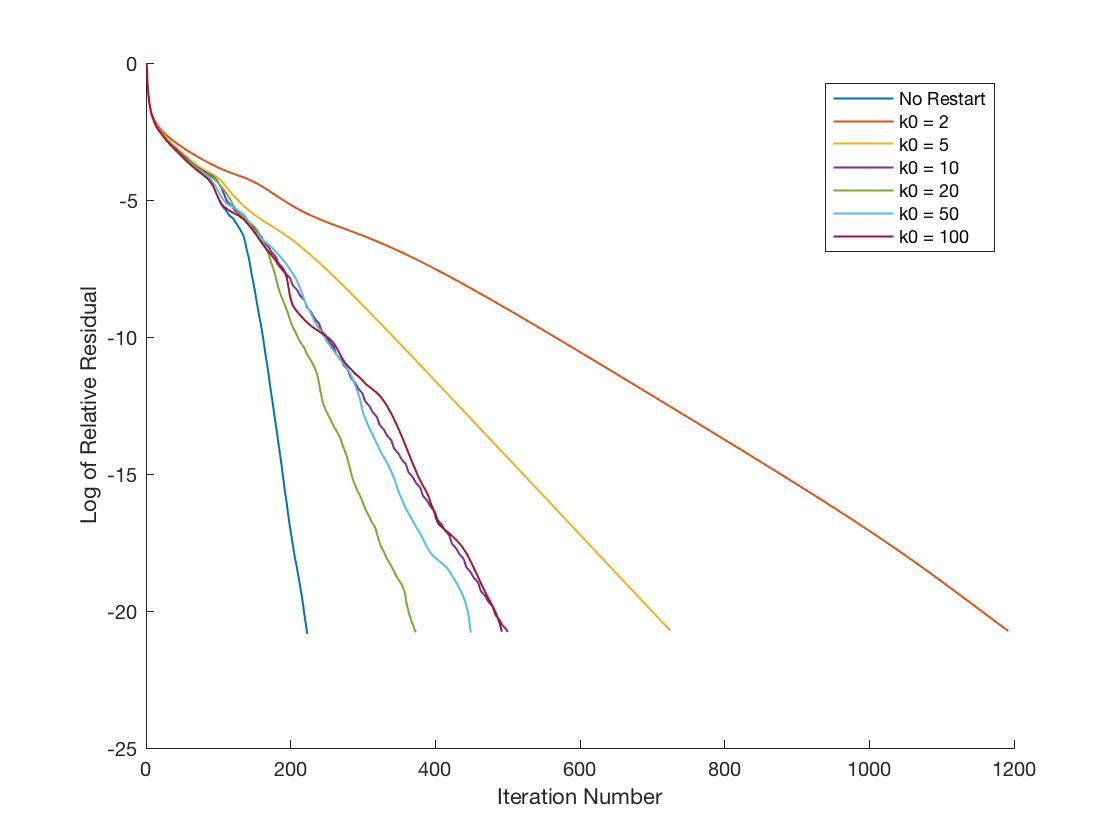
\includegraphics[scale=.39]{Prob3RelResidGraph.jpg}
\caption{Graph of Relative Residuals for Full and Restarted GMRES}
\end{figure}

\begin{table}[H]
%\centering
\renewcommand{\arraystretch}{1.3}
\hspace{-.2in}
\begin{small}
\begin{tabular}{| c || c | c | c | c | c | c | c |}
\hline
  & Full &  $k_0=2$ & $k_0=5$ & $k_0=10$ & $k_0=20$ & $k_0=50$ & $k_0=100$ \\
\hline 
\hline
\textbf{Outer} & 1 & 596 & 145 & 50 & 19 & 9 & 5 \\
\textbf{Inner} & 222 & 1 & 4 & 9 & 12 & 48 & 91 \\
\hline
\textbf{GMRES Steps} & 222 & 1191 & 724 & 499 & 372 & 448 & 491 \\
\textbf{\# of Matrix-Vector Products} & 223 & 1787 & 869 & 549 & 391 & 457 & 496 \\
\hline
\end{tabular}
\end{small}
\caption{Iteration Count and Matrix-Vector Product Totals for Full and Restarted GMRES}
\end{table} 
\noindent
\underline{Note:} "Outer" and "Inner" refer to the last iterations that GMRES finished on, produced by "iter" in the Matlab GMRES function.  We compute the number of GMRES steps and the total number of matrix-vector products using the following relationships:
\begin{align*}
\text{\# of GMRES Steps} &= (\text{Outer}-1)k_0 + \text{Inner} \\
\text{Total Products} &= \text{\# of GMRES Steps} + \text{Outer}. \\
\end{align*}
\qed\\

%\bigskip\bigskip
\noindent
\begin{problem} Let $A \in\R^{n\times n}$ be a general nonsingular matrix written as
$$A = D_0 - F - G,$$
where $D_0$, $- F$, and $-G$ denotes the diagonal part, strictly lower-triangular part, and strictly upper-triangluar part of $A$, respectively.  Let $D\in\R^{n\times n}$ be a given nonsingular diagonal matrix and consider the SSOR-type preconditioner
$$M := (D-F)D^{-1}(D-G) = M_1 M_2, \text{ } M_1 :=(D-F)D^{-1}, \text{ } M_2:=D-G,$$
for the matrix $A$.  We denote by
$$A' := M_1^{-1}AM_2^{-1}$$
the corresponding preconditioned matrix.
\end{problem}
\begin{itemize}
\item[(a)] Show that
$$A' = D\bigg((D-G)^{-1} + (D-F)^{-1}\big(I + D_1(D-G)^{-1}\big)\bigg),$$
where $D_1:=D_0 - 2D$.\\

First, we see that $M_1^{-1} = D(D-F)^{-1}$ and $M_2^{-1} = (D-G)^{-1}$.  Second, note that $D_1=D_0 - 2D$ can be rewritten as $D_0=D_1 + 2D$.  Now, it follows that:
\begin{align}
A' &= M_1^{-1}AM_2^{-1} \nonumber \\
&= D(D-F)^{-1}(D_0 - F - G)(D-G)^{-1} \nonumber \\
&= D\bigg((D-F)^{-1}(D_0 - F - G)(D-G)^{-1}\bigg) \nonumber \\
&= D\bigg((D-F)^{-1}(D_1 + 2D - F - G)(D-G)^{-1}\bigg) \nonumber \\
&= D\bigg((D-F)^{-1}\big(D_1 + (D- F) + (D - G)\big)(D-G)^{-1}\bigg) \nonumber \\
&=D\bigg( (D-F)^{-1}D_1(D-G)^{-1} + (D-F)^{-1}(D-F)(D-G)^{-1} + (D-F)^{-1}(D-G)(D-G)^{-1}\bigg) \nonumber \\
&= D\bigg((D-F)^{-1}D_1(D-G)^{-1} + (D-G)^{-1} + (D-F)^{-1}\bigg) \nonumber \\
&= D\bigg((D-G)^{-1} + (D-F)^{-1}\big(I + D_1(D-G)^{-1}\big)\bigg) \nonumber \text{ \checkmark} 
\end{align}
\qed\\


\item[(b)] Use the formula to derive an algorithm that computes matrix-vector products
$$q' = A'v', \text{ } v'\in\R^n,$$
as efficiently as possible.\\

\underline{Algorithm:}
\begin{itemize}
\item \underline{Input:} $D$, $F$, $G$, $D_0$, $D_1$, $v'$.
\item \underline{Output:} The matrix-vector product $q'=A'v'$.
\item Set $L=D-F$, $U=D-G$ and $D_1 = D_0 - 2D$.
\item (1) Use upper-triangular solver to solve $Uz=v'$ ($us = U\backslash z$).
\item (2) 1 matrix-vector product $d = D_1*us$.
\item (3) 1 SAXPY to compute $v = v' + d$.
\item (4) Use lower-triangular solver to solve $Ly=v$ ($ls=L\backslash v$.
\item (5) 1 SAXPY to compute $sum = ls + us$.
\item (6) 1 matrix-vector product $A'v' = D*sum$.
\end{itemize}

\lstset{language=matlab,frame=single}
\begin{lstlisting}[caption=Matlab Implementation of the Above Algorithm]
function Avp = ApMultFunct(L,U,D,D1,z)

us = U\z;
d = diag(D1).*us;
v = z + d;
ls = L\v;
sum = ls + us;
Avp = D*sum;
end
\end{lstlisting}\qed\\


\item[(c)] Let $m$ denote the number of nonzero off-diagonal entries $a_{jk}\neq 0$, $j\neq k$, of $A$.  Assuming that $v' \in\R^n$ is a vector with all nonzero entries, give an exact flop count (in terms of $n$ and $m$) for computing $q'=A'v'$ with your algorithm from part (b).\\

\newpage
\underline{Flop Count:}
\begin{itemize}
\item (1) For an upper-triangular solve, we need $n$ flops for multiplying the diagonals, $m$ flops for multiplying the non-zero off-diagonal entries, and $m$ flops for adding$\backslash$ subtracting $=n + 2m$ flops.
\item (2) Since $D_1$ is diagonal, then the matrix-vector product can be treated as a $n\times 1$ vector-vector product = $n$ flops.
\item (3) Addition of two $n\times 1$ vectors = $n$ flops.
\item (4) For a lower-triangular solve, we need $n$ flops for multiplying the diagonals, $m$ flops for multiplying the non-zero off-diagonal entries, and $m$ flops for adding$\backslash$ subtracting $=n + 2m$ flops.
\item (5) Addition of two $n\times 1$ vectors = $n$ flops.
\item (6) Since $D$ is diagonal, then the matrix-vector product can be treated as a $n\times 1$ vector-vector product = $n$ flops.
\item \textbf{Total Flops:} $6n + 4m$ flops.
\end{itemize}\qed
\end{itemize}


%\bigskip\bigskip
\noindent
\begin{problem}
\end{problem}
\begin{itemize}
\item[(a)] Use Matlab's function "gmres" to write Matlab programs for each of the following algorithms for solving linear systems:
\begin{itemize}
\item[(i)] GMRES (without preconditioning);
\item[(ii)] Restarted GMRES (without preconditioning);
\item[(iii)] GMRES with diagonal preconditioning applied from the right, i.e.,
$$M_1 = I \text{ and } M_2 = D_0,$$
where $D_0$ denotes the diagonal part of $A$;
\item[(iv)] Restarted GMRES with diagonal preconditioning applied from the right;
\item[(v)] GMRES with the SSOR-type preconditioner derived in problem 4;
\item[(vi)] Restarted GMRES with the SSOR-type preconditioner derived in problem 4;\\
\end{itemize}

\newpage
\lstset{language=matlab,frame=single}
\begin{lstlisting}[caption=Function to Run Full and Restarted GMRES with Preconditioning Option]
function x = GRMESrestartOpt(fileNum)

if (fileNum == 1)
    load('HW4_Problem5b_1.mat')
elseif (fileNum == 2)
    load('HW4_Problem5b_2.mat')
end

n = length(b);
x0 = ones(n,1);
maxit = n;
tol = 1e-8;
k0Vec = [5,10,20];

% Case 1: GMRES without preconditioning
[x,flag,relres,iter,resvec] = gmres(A,b,[],tol,maxit,[],[],x0);
iter
rel_resid = resvec./resvec(1);
k = (1:length(rel_resid));

hold on
subplot(4,2,1)
plot(k,log(rel_resid),'LineWidth',1)
xlabel('Iteration Number')
ylabel('Log of Relative Residual')
title('Full GMRES, No Preconditioning')

% Case 2: Restarted GMRES without preconditioning
k0Vec = [5,10,20];
for i=1:length(k0Vec)
    k0=k0Vec(i);
    [x,flag,relres,iter,resvec] = gmres(A,b,k0,tol,maxit,[],[],x0);
    iter
    rel_resid = resvec./resvec(1);
    k = (1:length(rel_resid));

    subplot(4,2,2)
    hold on
    plot(k,log(rel_resid),'LineWidth',1)
    xlabel('Iteration Number')
    ylabel('Log of Relative Residual')
    title('Restarted GMRES, No Preconditioning')
end
hold off
legend('k0 = 5','k0 = 10','k0 = 20')

% Case 3: GMRES with diagonal preconditioning applied from the right
D0 = diag(diag(A));
I = speye(n);
[x,flag,relres,iter,resvec] = gmres(A,b,[],tol,maxit,I,D0,x0);
iter
rel_resid = resvec./resvec(1);
k = (1:length(rel_resid));

subplot(4,2,3)
plot(k,log(rel_resid),'LineWidth',1)
xlabel('Iteration Number')
ylabel('Log of Relative Residual')
title('Full GMRES, With Diagonal Preconditioning')
    
% Case 4: Restarted GMRES with diagonal preconditioning applied from the
% right
for i=1:length(k0Vec)
    k0=k0Vec(i);
    [x,flag,relres,iter,resvec] = gmres(A,b,k0,tol,maxit,I,D0,x0);
    iter
    rel_resid = resvec./resvec(1);
    k = (1:length(rel_resid));

    subplot(4,2,4)
    hold on
    plot(k,log(rel_resid),'LineWidth',1)
    xlabel('Iteration Number')
    ylabel('Log of Relative Residual')
    title('Restarted GMRES, With Diagonal Preconditioning')
end
hold off
legend('k0 = 5','k0 = 10','k0 = 20')

% Case 5: Full GMRES with SSOR-type preconditioning (from problem 4)
D0 = diag(diag(A));
F = -tril(A,-1);
G = -triu(A,1);
I = speye(n);

%D=D0;
D = D0;
maxit = n;
D1 = D0 - 2*D;
L = D-F;
U = D-G;
M1 = L*D^(-1);
M2 = U;
bp = M1\b;
x0p = M2*x0;
% if we want the actual solution x_k, need to multiply it on the right by
% M2^-1 at the end

[x,flag,relres,iter,resvec] = gmres(@(v) ApMultFunct(L,U,D,D1,v),...
	bp,[],tol,maxit,[],[],x0p);
iter
rel_resid = resvec./resvec(1);
k = (1:length(rel_resid));

subplot(4,2,5)
plot(k,log(rel_resid),'LineWidth',1)
xlabel('Iteration Number')
ylabel('Log of Relative Residual')
title('Full GMRES, With SSOR-type Preconditioning, with D=D0')   

% D=10I
D = 10*I;
D1 = D0 - 2*D;
L = D-F;
U = D-G;
M1 = L*D^(-1);
M2 = U;
bp = M1\b;
x0p = M2*x0;
    
[x,flag,relres,iter,resvec] = gmres(@(v) ApMultFunct(L,U,D,D1,v),...
	bp,[],tol,maxit,[],[],x0p);
iter
rel_resid = resvec./resvec(1);
k = (1:length(rel_resid));

subplot(4,2,6)
plot(k,log(rel_resid),'LineWidth',1)
xlabel('Iteration Number')
ylabel('Log of Relative Residual')
title('Full GMRES, With SSOR-type Preconditioning, with D=10I')

% Case 6: Restarted GMRES with SSOR-type preconditioning
%D=D0
D = D0;
maxit = n;
D1 = D0 - 2*D;
L = D-F;
U = D-G;
M1 = L*D^(-1);
M2 = U;
bp = M1\b;
x0p = M2*x0;

for i=1:length(k0Vec)
    k0=k0Vec(i); 

    [x,flag,relres,iter,resvec] = gmres(@(v) ApMultFunct(L,U,D,D1,v),...
    	bp,k0,tol,maxit,[],[],x0p);
    iter
    rel_resid = resvec./resvec(1);
    k = (1:length(rel_resid));

    subplot(4,2,7)
    hold on
    plot(k,log(rel_resid),'LineWidth',1)
    xlabel('Iteration Number')
    ylabel('Log of Relative Residual')
    title('Restarted GMRES, With SSOR-type Preconditioning, with D = D0')
end
hold off
legend('k0 = 5','k0 = 10','k0 = 20')
 
%D=10I
D = 10*I;
D1 = D0 - 2*D;
L = D-F;
U = D-G;

M1 = L*D^(-1);
M2 = U;
bp = M1\b;
x0p = M2*x0;

for i=1:length(k0Vec)
    k0=k0Vec(i); 

    [x,flag,relres,iter,resvec] = gmres(@(v) ApMultFunct(L,U,D,D1,v),...
    	bp,k0,tol,maxit,[],[],x0p);
    iter
    rel_resid = resvec./resvec(1);
    k = (1:length(rel_resid));

    subplot(4,2,8)
    hold on
    plot(k,log(rel_resid),'LineWidth',1)
    xlabel('Iteration Number')
    ylabel('Log of Relative Residual')
    title('Restarted GMRES, With SSOR-type Preconditioning, with D = 10I')
end
hold off
legend('k0 = 5','k0 = 10','k0 = 20') 
end
\end{lstlisting}


\item[(b)] Use your Matlab programs to solve the two linear systems provided in the Matlab files $"HW4\_Problem5b\_1.mat"$ and $"HW4\_Problem5b\_2.mat"$.  For both systems, choose the vector $x_0 = e\in\R^n$ of all $1$'s as initial guess and try to solve the system to relative residual norm of $tol = 10^{-8}$.  Run algorithms (v) and (vi) with these two choices of $D$: $D=D_0$ and $D=10I$.  Use the restarted parameters $k_0=5$, $k_0=10$, and $k_0=20$ for algorithms (ii), (iv), and (vi).\\
\end{itemize}


% graphs for file 1
\begin{figure}[H]
%\center
\hspace{-.3in}
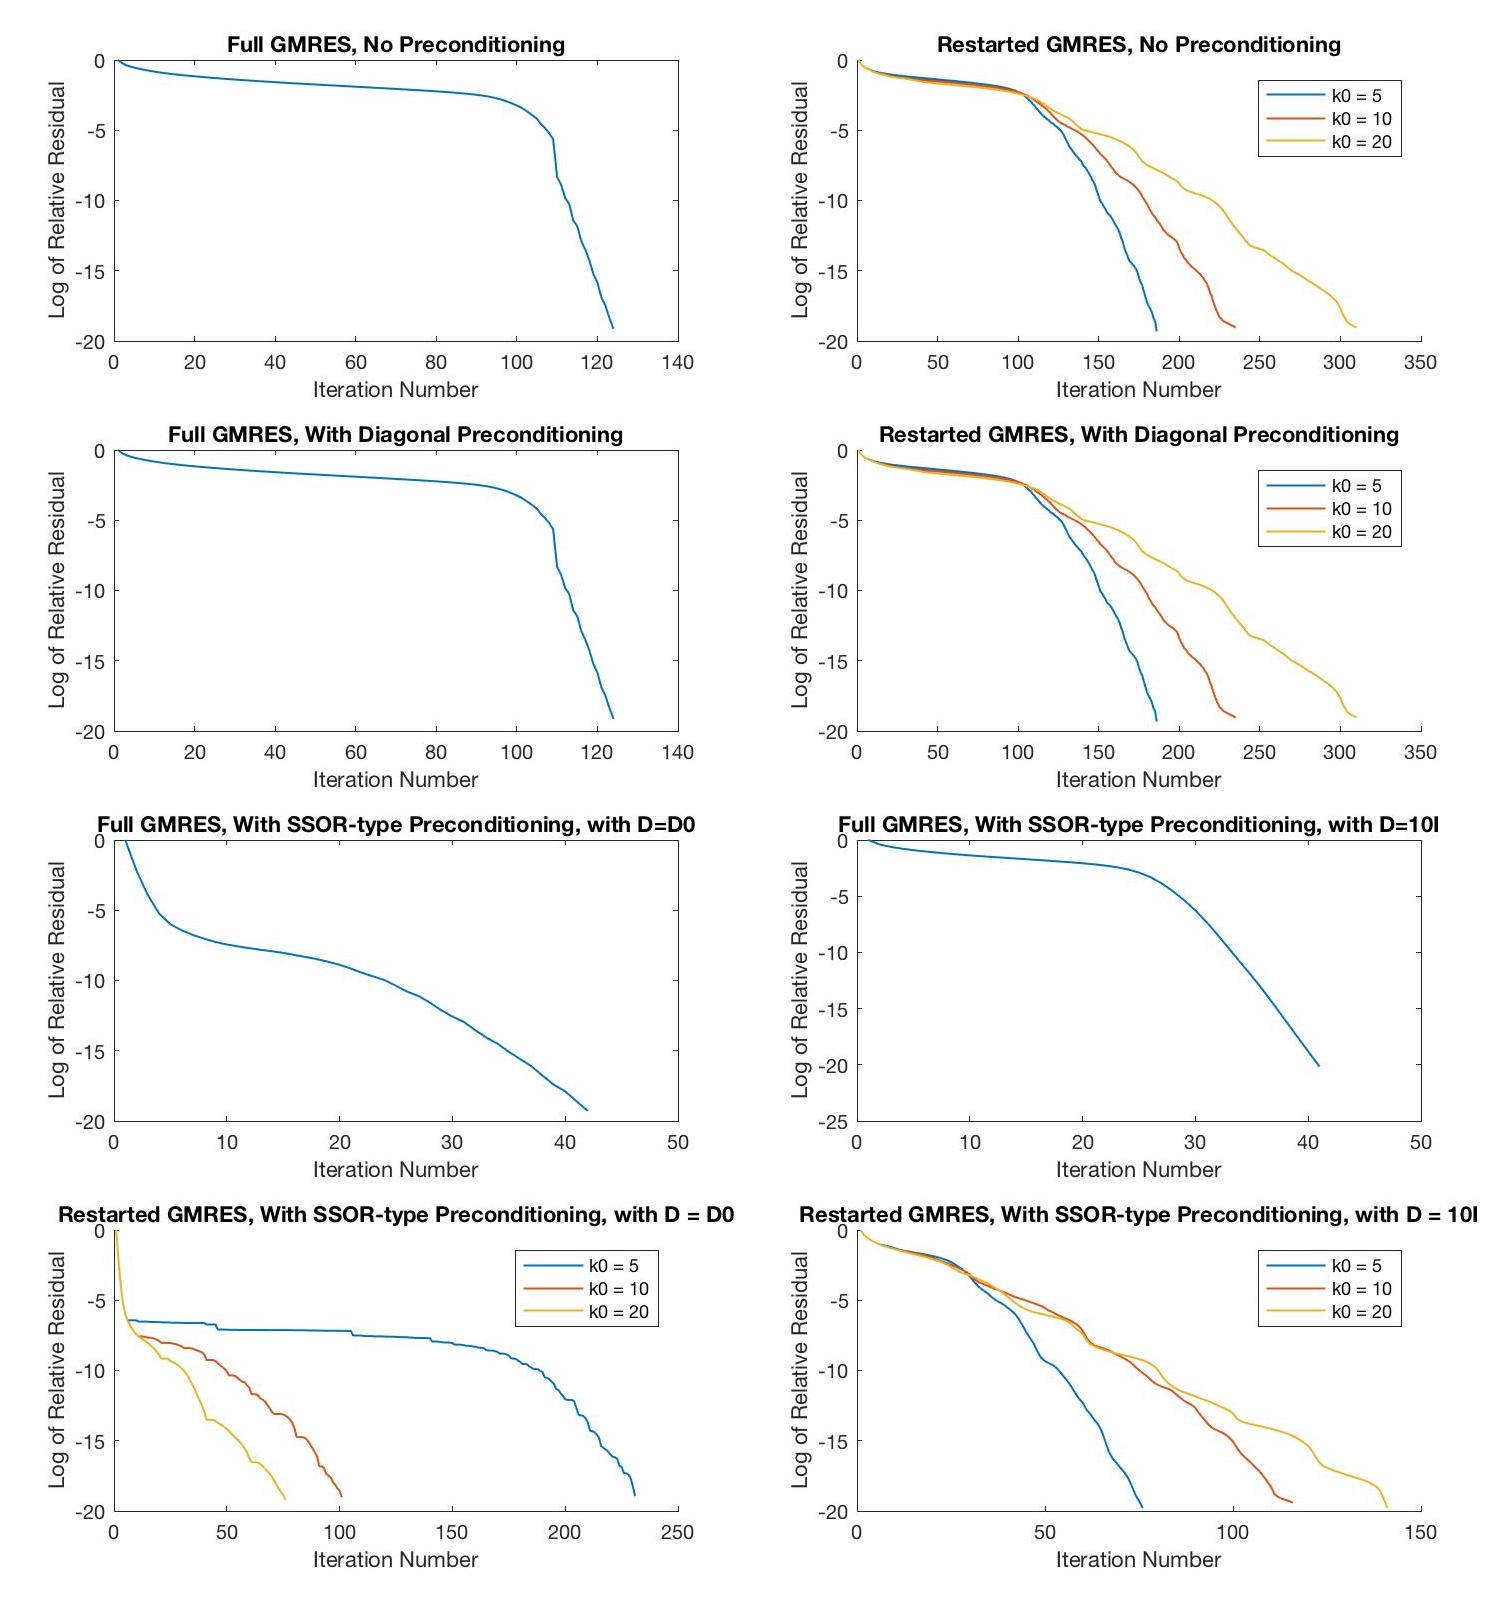
\includegraphics[scale=.33]{Prob5Set1Graphs.jpg}
\caption{Graphs of Relative Residuals For GMRES with and without Restart for Data Set 1}
\end{figure}

\begin{table}[H]
%\centering
\renewcommand{\arraystretch}{1.3}
\hspace{-.35in}
\begin{small}
\begin{tabular}{| c || c | c | c | c | c || c | c |}
\hline
\textbf{Case} &  \textbf{Full/Restart} & \textbf{Preconditioning} & \textbf{$k_0$} & \textbf{Outer} & \textbf{Inner} & \textbf{GMRES Steps} & \textbf{Total Products}\\
\hline 
\hline
(i)  & Full & No & - & 1 & 123 & 123 & 124  \\
\hline
(ii) & Restarted & No & 5 & 37 & 5 & 185 &  222\\
  &  &  & 10 & 24 & 4 & 234 &  258\\
  &  &  & 20 & 16 & 9 & 309 &  325\\
\hline
(iii) & Full & Diagonal & - & 1 & 123 & 123 & 124 \\
\hline
(iv) & Restarted & Diagonal & 5 & 37 & 5 & 185 &  222\\
  &  &  & 10 & 24 & 4 & 234 &  258\\
  &  &  & 20 & 16 & 9 & 309 &  325\\
\hline
(v) & Full & SSOR ($D=D_0$) & - & 1 & 41 & 41 & 42 \\
\hline
 & Full & SSOR ($D=10I$) & - & 1 & 40 & 40 & 41 \\
\hline
(vi) & Restarted & SSOR ($D=D_0$) & 5 & 46 & 5 & 230 &  276\\
  &  &  & 10 & 10 & 10 & 100 &  110\\
  &  &  & 20 & 4 & 15 & 75 & 79\\
\hline
 & Restarted & SSOR ($D=10I$) & 5 & 15 & 5 & 75 &  90\\
  &  &  & 10 & 12 & 5 & 115 &  127\\
  &  &  & 20 & 7 & 20 & 140 &  147\\
\hline
\end{tabular}
\end{small}
\caption{Iteration Count and Matrix-Vector Product Totals for $"HW4\_Problem5b\_1.mat"$}
\end{table}
\noindent
\underline{Note:} "Outer" and "Inner" refer to the last iterations that GMRES finished on, produced by "iter" in the Matlab GMRES function.  We compute the number of GMRES steps and the total number of matrix-vector products using the following relationships:
\begin{align*}
\text{\# of GMRES Steps} &= (\text{Outer}-1)k_0 + \text{Inner} \\
\text{Total Products} &= \text{\# of GMRES Steps} + \text{Outer}. \\
\end{align*}
\\


% grpahs for file 2
\begin{figure}[H]
%\center
\hspace{-.3in}
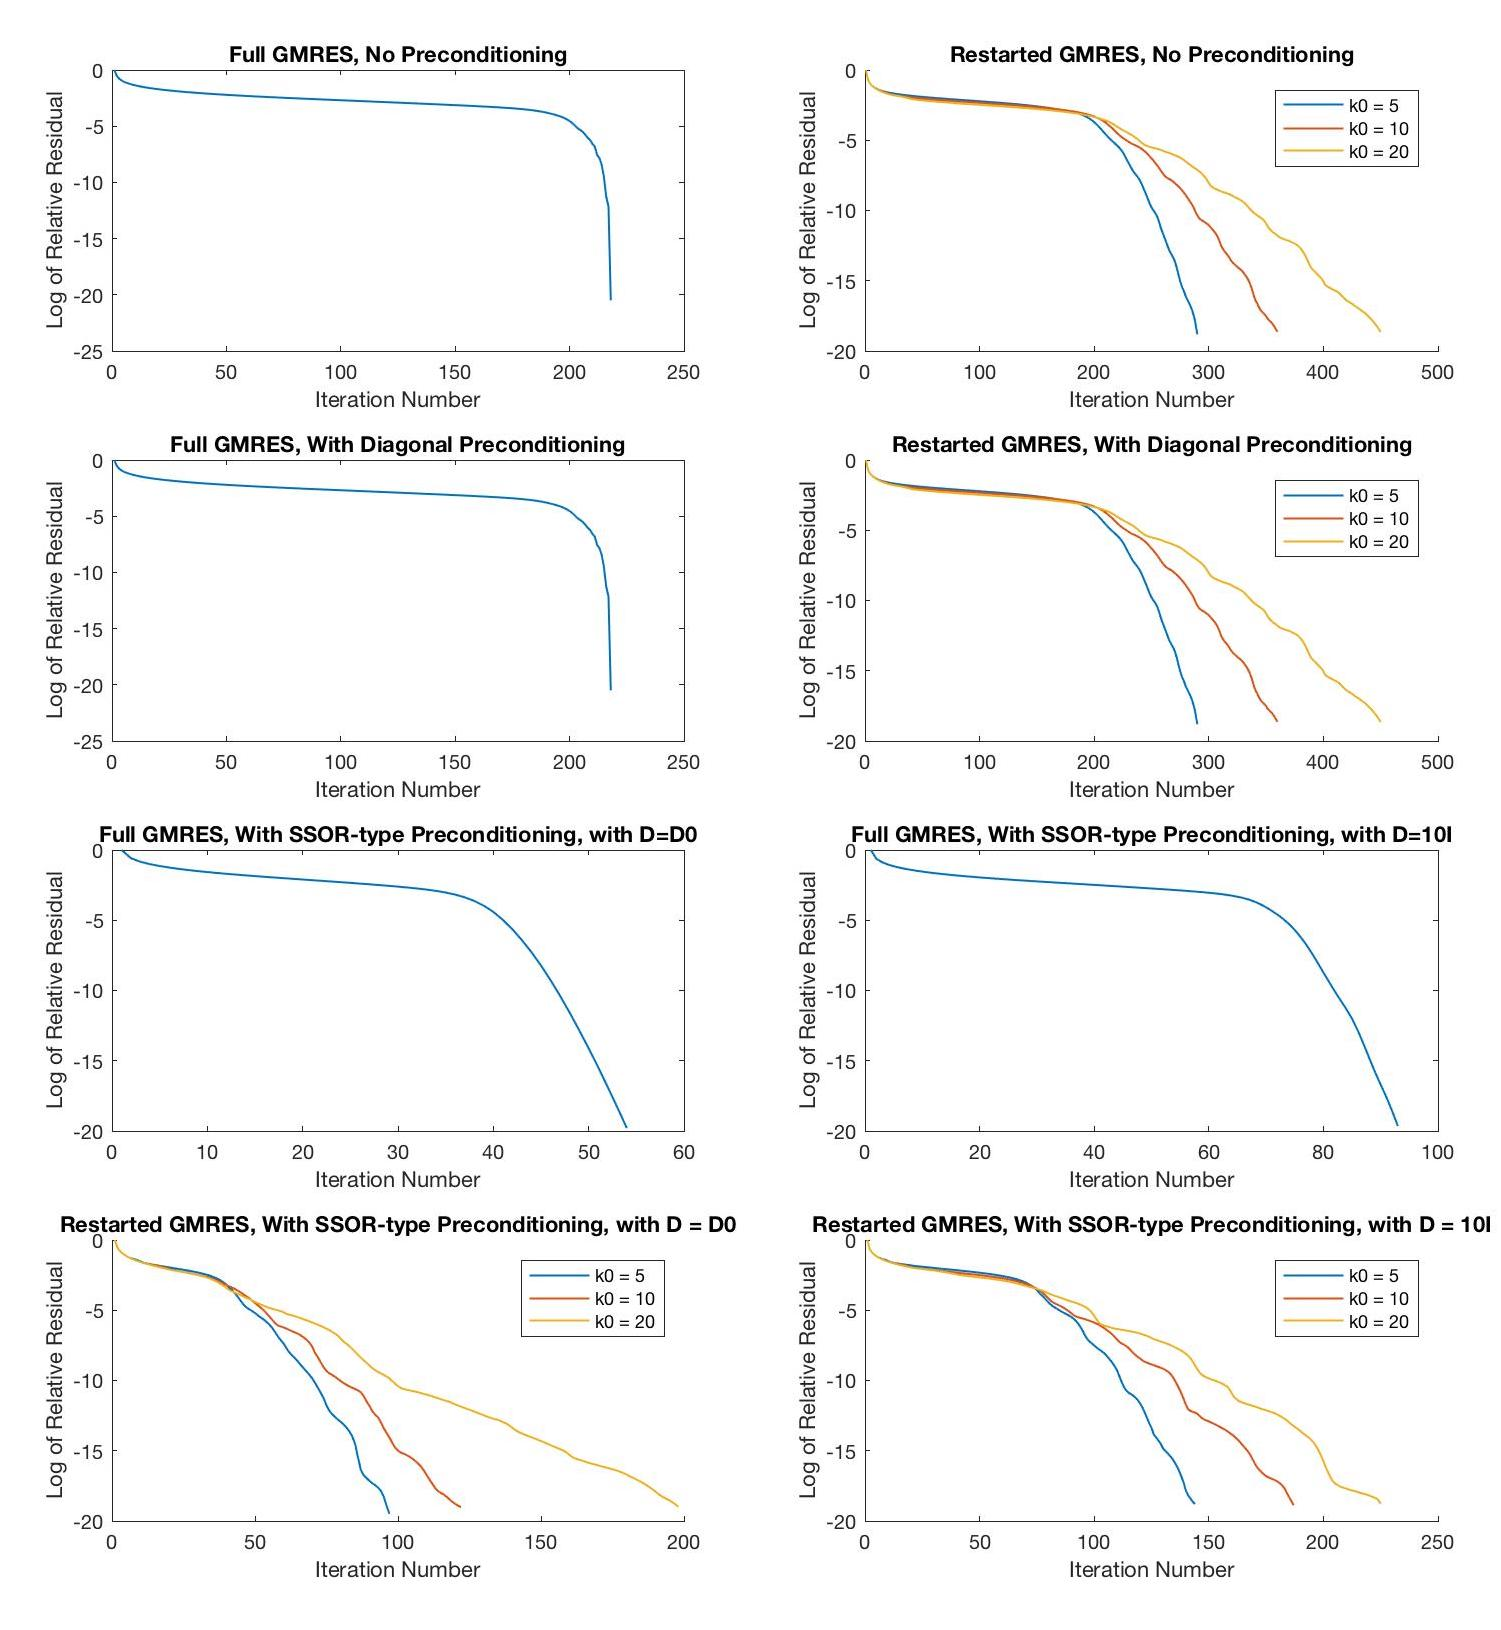
\includegraphics[scale=.33]{Prob5Set2Graphs.jpg}
\caption{Graphs of Relative Residuals For GMRES with and without Restart for Data Set 2}
\end{figure}


\begin{table}[H]
%\centering
\renewcommand{\arraystretch}{1.3}
\hspace{-.35in}
\begin{small}
\begin{tabular}{| c || c | c | c | c | c || c | c |}
\hline
\textbf{Case} &  \textbf{Full/Restart} & \textbf{Preconditioning} & \textbf{$k_0$} & \textbf{Outer} & \textbf{Inner} & \textbf{GMRES Steps} & \textbf{Total Products}\\
\hline 
\hline
(i)  & Full & No & - & 1 & 217 & 217 & 218 \\
\hline
(ii) & Restarted & No & 5 & 58 & 4 & 289 &  347\\
  &  &  & 10 & 36 & 9 & 359 &  395\\
  &  &  & 20 & 23 & 9 & 449 &  472\\
\hline
(iii) & Full & Diagonal & - & 1 & 217 & 217 & 218 \\
\hline
(iv) & Restarted & Diagonal & 5 & 58 & 4 & 289 &  347\\
  &  &  & 10 & 36 & 9 & 359 &  395\\
  &  &  & 20 & 23 & 9 & 449 &  472\\
\hline
(v) & Full & SSOR ($D=D_0$) & - & 1 & 53 & 53 & 54 \\
\hline
 & Full & SSOR ($D=10I$) & - & 1 & 92 & 92 & 93 \\
\hline
(vi) & Restarted & SSOR ($D=D_0$) & 5 & 20 & 1 & 96 & 116\\
  &  &  & 10 & 13 & 1 & 121 &  134\\
  &  &  & 20 & 10 & 17 & 197 &  207\\
\hline
 & Restarted & SSOR ($D=10I$) & 5 & 29 & 3 & 143 &  172\\
  &  &  & 10 & 19 & 6 & 186 & 205 \\
  &  &  & 20 & 12 & 4 & 224 &  236\\
\hline
\end{tabular}
\end{small}
\caption{Iteration Count and Matrix-Vector Product Totals for $"HW4\_Problem5b\_2.mat"$}
\end{table}
\noindent
\underline{Note:} "Outer" and "Inner" refer to the last iterations that GMRES finished on, produced by "iter" in the Matlab GMRES function.  We compute the number of GMRES steps and the total number of matrix-vector products using the following relationships:
\begin{align*}
\text{\# of GMRES Steps} &= (\text{Outer}-1)k_0 + \text{Inner} \\
\text{Total Products} &= \text{\# of GMRES Steps} + \text{Outer}. \\
\end{align*}
\qed\\






\end{document}

% insert Matlab code
\lstset{language=matlab,frame=single}
\begin{lstlisting}[caption=]

\end{lstlisting}

% import Matlab code directly
\lstinputlisting[style=Matlab-editor,basicstyle=\ttfamily\small]{codename.m}

% table template
\begin{table}[H]
\centering
\renewcommand{\arraystretch}{1.3}
\begin{small}
\begin{tabular}{| c | c |}
\hline
Result &  Value\\
\hline 

\hline
\end{tabular}
\end{small}
\caption{ }
\end{table} 

% insert jpeg
\begin{figure}[H]
\center
\includegraphics[scale=.39]{ .jpg}
\caption{ }
\end{figure}

% change text color
{\color{red} **colored text goes here}

% change the text size in math environment
\[\Scale[0.5]{y = \sin^2 x}\] 

% to put a colored box aroubd something. can change color
\begin{mybox}{red}{Title}
Stuff in box
\end{mybox}